\documentclass[11pt]{article}

\usepackage{graphicx}

% Construct the basic page sizes
\oddsidemargin  0.0in
\evensidemargin 0.0in
\textwidth      6.5in
\headheight     0.25in
\topmargin      0.0in
\textheight=8.5in


\begin{document}

\title{Program Flow for a Propagation Enabled Command}
\author{Darrel J. Conway\\\textit{Thinking Systems, Inc.}\\
Steven P. Hughes\\\textit{Goddard Space Flight Center}}
\date{December 4, 2008}
\maketitle

\begin{abstract}
This document described the interactions between the components used in GMAT to propagate objects.
\end{abstract}

\section{Introduction}

GMAT provides a collection of components that are tailored to advancing objects in GMAT's model over time.  Users instruct GMAT about the types of objects that are expected to evolve, and the elements of those objects that are needed by the model, using Mission Control Sequence commands that are enabled for propagation.  The current design plan for GMAT identifies three propagation-enabled commands: ``Propagate'', ``RunEstimator'', and ``RunSimulator''.  The discussion that follows will examine the Propagate command in detail, and then discuss the other commands in the context of propagation.

\section{Propagation Overview}

The commands governing propagation in GMAT all pass through five stages in the course of modeling a mission.  These stages, shown in Figure~\ref{fig:PropLifetime}, start from the creation of the command and run through its initialization, setup and execution, and completion and finalization.  The following paragraphs give an overview of each of these stages.

\begin{figure}[htb]
\begin{center}
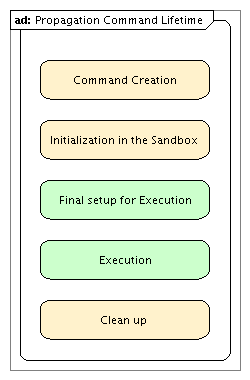
\includegraphics[width=2in]{Images/PropagationCommandLifetime.png}
\caption{Stages in the Lifetime of a Propagation Enabled Command}
\label{fig:PropLifetime}
\end{center}
\end{figure}

\paragraph{Command Creation}

Propagation enabled commands are created following the same pattern as all other commands in GMAT.  A user creates the command, either through a line if text in a mission script file or function file or from GMAT's graphical user interface using the panel for the command.  When the script is parsed or the panel closed, GMAT creates an object based on that action, and passes that object the detailed information necessary to configure the command.  This information is stored in string form at this stage.  It identifies the interconnections that are needed to execute the command during a mission run.  The command validates all of the information that can be checked locally at this point.

\paragraph{Initialization}

The first step GMAT performs when running a mission is the initialization step in the Sandbox used for the run.  During this phase of the run, all of the objects configured for the mission are cloned into the Sandbox, and the mission control sequence is assigned to the Sandbox.  The objects are initialized, and then each command in the control sequence is initialized.  During initialization, all of the interconnections between components are set, and as much preparation as possible is made to run the mission.  For propagation enabled commands, initialization includes cloning of the configured propagators used in the command so that a local instance is available for propagation.  The parameters needed to execute the desired propagation are set, and the data needed for propagation collected and validated.  The actual propagation state vector cannot be constructed at this point because commands in the mission control sequence prior to the propagation enabled command may affect that state vector.

\paragraph{Final Setup}

After initialization, the Sandbox starts running the Mission Control Sequence by executing the commands sequentially.  For propagation enabled commands, the first action taken when execution is requested is a final setup of the objects used for propagation.  This setup checks for changes to the objects that affect the propagation state (for example, a transient force like a thruster firing may have become active), builds the propagation state vector, establishes a mapping between the ODE model and that state vector if the propagator needs it, and populates the state vector with the initial data that is to be propagated.

\paragraph{Execution}

Once the final setup is complete, the command is ready to begin propagation.  Propagation is performed a step at a time.  The propagator is asked for an integration step.  The step is taken and the resulting state vector returned.  The command checks the result to see if a stopping point has been reached.  If not, the objects are updated with the propagated information.  If a stopping point was encountered in the propagation span, the command invokes stopping condition logic to propagate to the desired point.  The propagation enabled commands also perform periodic interrupts so that the Sandbox can check for user interrupts during propagation.

\paragraph{Finalization}

Once the command has completed execution, there are several final steps taken.  Settings on the command are updated to make it reentrant, so that if it is encountered inside of a loop, it can perform the final setup checks, make any required updates, and propagate again.  Data generated during execution are buffered at this point for display at user request.

The text above describes at a high level the process followed for all propagation enabled commands.  The next section provides a short definition of the components GMAT uses in the propagation subsystem.  Following that, the process performed for each of these five steps is described in detail for the Propagate command.  Additions for the remaining propagation enabled commands follow that section.

\section{Components used in Propagation}

Here I'll put in some descriptions of the prop state manager, PropSetup, etc.  Here's the list:

\begin{description}
\item[PropSetup ]
\item[Propagator]
\item[Integrator]
\item[ODEModel]
\item[PhysicalModel]
\item[GmatState]
\item[StateManager]
\item[PropagationStateManager]
\item[EstimationStateManager]
\item[SpacePoint]
\item[SpaceObject]
\end{description}

\section{The Propagate Command}

This document describes the interactions between commands and other objects used in GMAT's propagation code.  It is not intended to describe the full set of features implemented in the Propagate command itself; those details can be found in GMAT's Architectural Specification\cite{GMAT:2008}, in the chapter entitled "Specific Command Details."  

The Propagate command is the prototypical propagation enabled command.  As such, it is used here to describe how the objects in GMAT interact to propagate an element of a mission.  The following script will be used when examples are needed in the discussion:

\begin{quote}
\begin{verbatim}
Create Spacecraft sat;

Create ForceModel fm;
fm.PrimaryBodies = {Earth};
fm.PointMasses = {Luna, Sun};
fm.Drag = MSISE90;
fm.SRP = On;

Create Propagator prop;
prop.FM = fm;
prop.Type = PrinceDormand78;

Propagate prop(sat, 'STM');
\end{verbatim}
\end{quote}

\noindent The script defines three objects: a Spacecraft named sat, a ForceModel named fm, and a PropSetup named prop.  Parameters are set on these objects where they may be useful for the discussion; where not useful, the default settings are used.

The following paragraphs describe the fives stages in the life of a Propagate command, using the sample script for illustrative purposes\footnote{The process followed from the GUI is identical from the perspective of the Propagate command, though a few details differ -- the use of a GuiInterpreter rather than a ScriptInterpreter, for instance.  The interactive nature of the GUI makes providing the information about how the internal objects interact unnecessarily complicated.}.

\subsection{Parsing: Propagation Specifics}

TBWD  (To be written and drawn)

\subsection{Initialization in the Sandbox}

\begin{figure}[htb] 
   \centering
   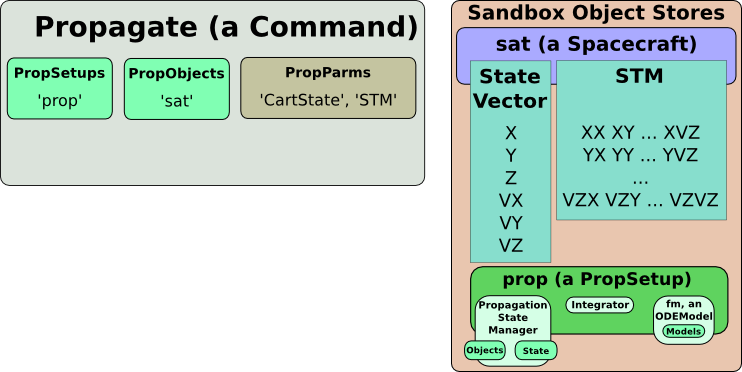
\includegraphics[width=5.5in]{Images/PersistenceStart.png} 
   \caption{Objects at the Start of the Propagate Command Initialization}
   \label{fig:PersistenceStart}
\end{figure}

Initialization for the Propagate command occurs after all of the resources defined in the script have been cloned into the Sandbox and initialized.  The objects relevant to the command initialization are shown in Figure~\ref{fig:PersistenceStart}.  The Sandbox object stores contain the Spacecraft and PropSetup instances named as objects needed by the Propagate command.  Pointers to these object stores are passed into the Propagate command immediately before the command is initialized.  Then the initialization process is executed by a call from the Sandbox to the Propagate command's Initialize() method.

The steps followed in the Initialize() method are shown in Figure~\ref{fig:PropagateInitialize}.

\begin{figure}[p] 
   \centering
   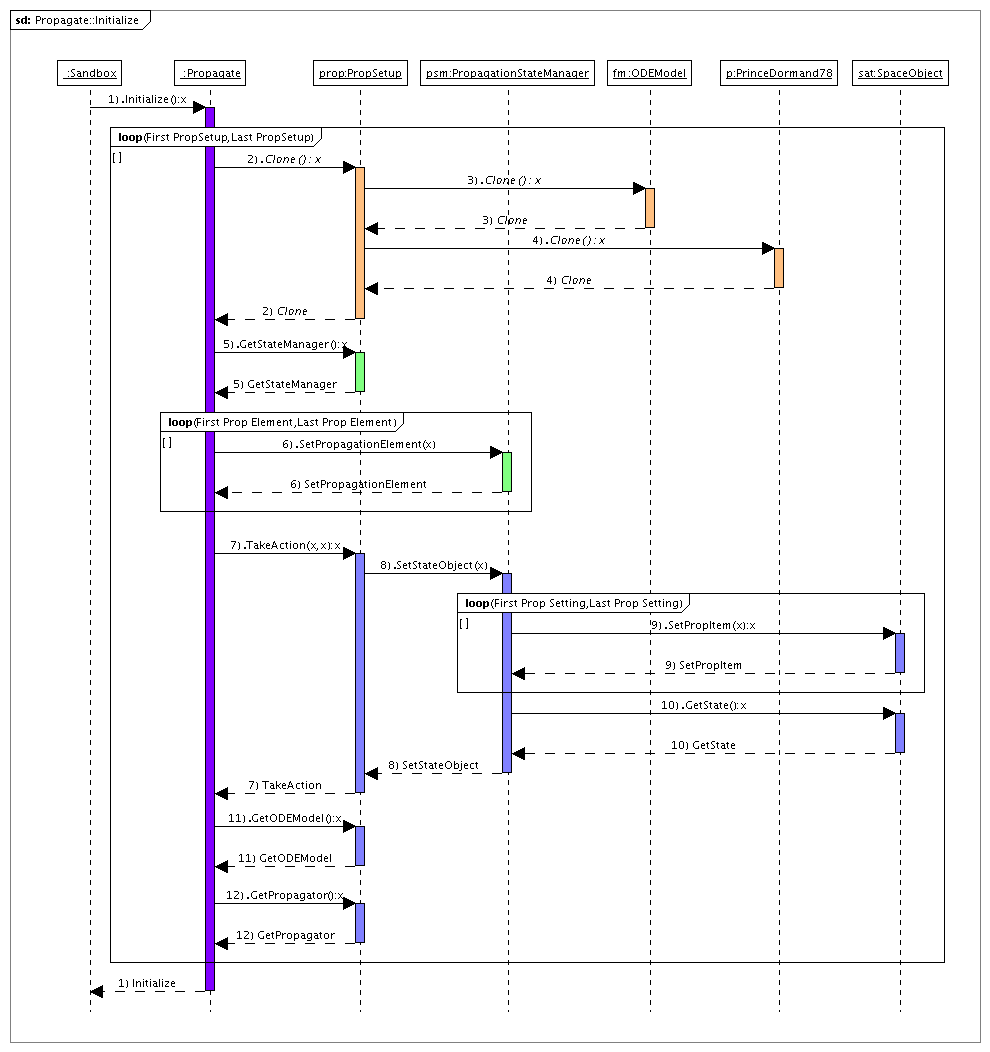
\includegraphics[width=6.5in]{Images/PropagateInitialize.png} 
   \caption{Steps Followed in the Propagate Command Initialization}
   \label{fig:PropagateInitialize}
\end{figure}

\begin{figure}[htb] 
   \centering
   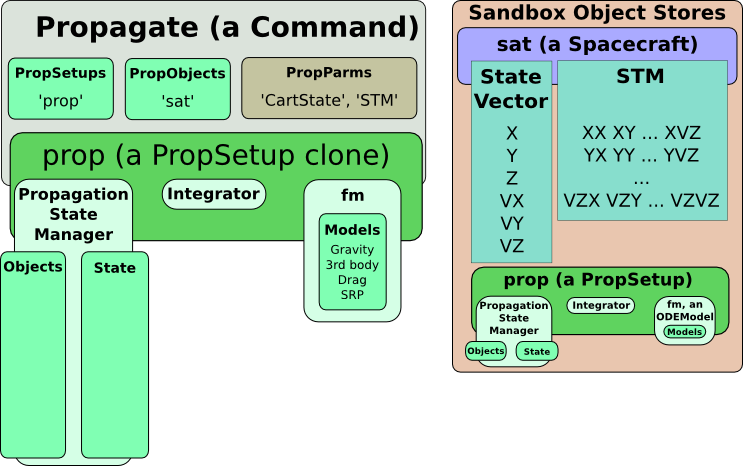
\includegraphics[width=5.5in]{Images/PersistenceCloned.png} 
   \caption{Objects after the Propagate Command Cloning}
   \label{fig:PersistenceCloned}
\end{figure}

\subsection{Preparing for Execution}

\subsection{Execution}

\subsection{Finishing Up}

\section{The RunEstimator Command}

\section{The RunSimulator Command}

\begin{thebibliography}{99}

    %-------------------------------------
    %  Guidance Papers
    %-------------------------------------

    \bibitem{GMAT:2008} The GMAT Development Team, \textbf{General Mission Analysis Tool (GMAT) Architectural Specification}, 2008.

\end{thebibliography}

\end{document}
